% Options for packages loaded elsewhere
\PassOptionsToPackage{unicode}{hyperref}
\PassOptionsToPackage{hyphens}{url}
%
\documentclass[
]{article}
\usepackage{amsmath,amssymb}
\usepackage{lmodern}
\usepackage{iftex}
\ifPDFTeX
  \usepackage[T1]{fontenc}
  \usepackage[utf8]{inputenc}
  \usepackage{textcomp} % provide euro and other symbols
\else % if luatex or xetex
  \usepackage{unicode-math}
  \defaultfontfeatures{Scale=MatchLowercase}
  \defaultfontfeatures[\rmfamily]{Ligatures=TeX,Scale=1}
\fi
% Use upquote if available, for straight quotes in verbatim environments
\IfFileExists{upquote.sty}{\usepackage{upquote}}{}
\IfFileExists{microtype.sty}{% use microtype if available
  \usepackage[]{microtype}
  \UseMicrotypeSet[protrusion]{basicmath} % disable protrusion for tt fonts
}{}
\makeatletter
\@ifundefined{KOMAClassName}{% if non-KOMA class
  \IfFileExists{parskip.sty}{%
    \usepackage{parskip}
  }{% else
    \setlength{\parindent}{0pt}
    \setlength{\parskip}{6pt plus 2pt minus 1pt}}
}{% if KOMA class
  \KOMAoptions{parskip=half}}
\makeatother
\usepackage{xcolor}
\IfFileExists{xurl.sty}{\usepackage{xurl}}{} % add URL line breaks if available
\IfFileExists{bookmark.sty}{\usepackage{bookmark}}{\usepackage{hyperref}}
\hypersetup{
  pdftitle={Patterns of occurrence},
  pdfauthor={Dr.~Shai Pilosof, Ecological Complexity Lab www.bgu.ac.il/ecomplab, Ben Gurion University, Israel},
  hidelinks,
  pdfcreator={LaTeX via pandoc}}
\urlstyle{same} % disable monospaced font for URLs
\usepackage[margin=1in]{geometry}
\usepackage{color}
\usepackage{fancyvrb}
\newcommand{\VerbBar}{|}
\newcommand{\VERB}{\Verb[commandchars=\\\{\}]}
\DefineVerbatimEnvironment{Highlighting}{Verbatim}{commandchars=\\\{\}}
% Add ',fontsize=\small' for more characters per line
\usepackage{framed}
\definecolor{shadecolor}{RGB}{248,248,248}
\newenvironment{Shaded}{\begin{snugshade}}{\end{snugshade}}
\newcommand{\AlertTok}[1]{\textcolor[rgb]{0.94,0.16,0.16}{#1}}
\newcommand{\AnnotationTok}[1]{\textcolor[rgb]{0.56,0.35,0.01}{\textbf{\textit{#1}}}}
\newcommand{\AttributeTok}[1]{\textcolor[rgb]{0.77,0.63,0.00}{#1}}
\newcommand{\BaseNTok}[1]{\textcolor[rgb]{0.00,0.00,0.81}{#1}}
\newcommand{\BuiltInTok}[1]{#1}
\newcommand{\CharTok}[1]{\textcolor[rgb]{0.31,0.60,0.02}{#1}}
\newcommand{\CommentTok}[1]{\textcolor[rgb]{0.56,0.35,0.01}{\textit{#1}}}
\newcommand{\CommentVarTok}[1]{\textcolor[rgb]{0.56,0.35,0.01}{\textbf{\textit{#1}}}}
\newcommand{\ConstantTok}[1]{\textcolor[rgb]{0.00,0.00,0.00}{#1}}
\newcommand{\ControlFlowTok}[1]{\textcolor[rgb]{0.13,0.29,0.53}{\textbf{#1}}}
\newcommand{\DataTypeTok}[1]{\textcolor[rgb]{0.13,0.29,0.53}{#1}}
\newcommand{\DecValTok}[1]{\textcolor[rgb]{0.00,0.00,0.81}{#1}}
\newcommand{\DocumentationTok}[1]{\textcolor[rgb]{0.56,0.35,0.01}{\textbf{\textit{#1}}}}
\newcommand{\ErrorTok}[1]{\textcolor[rgb]{0.64,0.00,0.00}{\textbf{#1}}}
\newcommand{\ExtensionTok}[1]{#1}
\newcommand{\FloatTok}[1]{\textcolor[rgb]{0.00,0.00,0.81}{#1}}
\newcommand{\FunctionTok}[1]{\textcolor[rgb]{0.00,0.00,0.00}{#1}}
\newcommand{\ImportTok}[1]{#1}
\newcommand{\InformationTok}[1]{\textcolor[rgb]{0.56,0.35,0.01}{\textbf{\textit{#1}}}}
\newcommand{\KeywordTok}[1]{\textcolor[rgb]{0.13,0.29,0.53}{\textbf{#1}}}
\newcommand{\NormalTok}[1]{#1}
\newcommand{\OperatorTok}[1]{\textcolor[rgb]{0.81,0.36,0.00}{\textbf{#1}}}
\newcommand{\OtherTok}[1]{\textcolor[rgb]{0.56,0.35,0.01}{#1}}
\newcommand{\PreprocessorTok}[1]{\textcolor[rgb]{0.56,0.35,0.01}{\textit{#1}}}
\newcommand{\RegionMarkerTok}[1]{#1}
\newcommand{\SpecialCharTok}[1]{\textcolor[rgb]{0.00,0.00,0.00}{#1}}
\newcommand{\SpecialStringTok}[1]{\textcolor[rgb]{0.31,0.60,0.02}{#1}}
\newcommand{\StringTok}[1]{\textcolor[rgb]{0.31,0.60,0.02}{#1}}
\newcommand{\VariableTok}[1]{\textcolor[rgb]{0.00,0.00,0.00}{#1}}
\newcommand{\VerbatimStringTok}[1]{\textcolor[rgb]{0.31,0.60,0.02}{#1}}
\newcommand{\WarningTok}[1]{\textcolor[rgb]{0.56,0.35,0.01}{\textbf{\textit{#1}}}}
\usepackage{graphicx}
\makeatletter
\def\maxwidth{\ifdim\Gin@nat@width>\linewidth\linewidth\else\Gin@nat@width\fi}
\def\maxheight{\ifdim\Gin@nat@height>\textheight\textheight\else\Gin@nat@height\fi}
\makeatother
% Scale images if necessary, so that they will not overflow the page
% margins by default, and it is still possible to overwrite the defaults
% using explicit options in \includegraphics[width, height, ...]{}
\setkeys{Gin}{width=\maxwidth,height=\maxheight,keepaspectratio}
% Set default figure placement to htbp
\makeatletter
\def\fps@figure{htbp}
\makeatother
\setlength{\emergencystretch}{3em} % prevent overfull lines
\providecommand{\tightlist}{%
  \setlength{\itemsep}{0pt}\setlength{\parskip}{0pt}}
\setcounter{secnumdepth}{-\maxdimen} % remove section numbering
\ifLuaTeX
  \usepackage{selnolig}  % disable illegal ligatures
\fi

\title{Patterns of occurrence}
\usepackage{etoolbox}
\makeatletter
\providecommand{\subtitle}[1]{% add subtitle to \maketitle
  \apptocmd{\@title}{\par {\large #1 \par}}{}{}
}
\makeatother
\subtitle{Supplementary Infomation for the paper:}
\author{Dr.~Shai Pilosof, Ecological Complexity Lab
\url{www.bgu.ac.il/ecomplab}, Ben Gurion University, Israel}
\date{2022-03}

\begin{document}
\maketitle

\begin{Shaded}
\begin{Highlighting}[]
\CommentTok{\# Includes {-}{-}{-}{-}{-}{-}{-}{-}{-}{-}{-}{-}}
\FunctionTok{library}\NormalTok{(tidyverse)}
\FunctionTok{library}\NormalTok{(magrittr)}
\FunctionTok{library}\NormalTok{(cowplot)}
\FunctionTok{library}\NormalTok{(reshape2) }
\FunctionTok{library}\NormalTok{(vegan)}
\FunctionTok{library}\NormalTok{(igraph)}
\FunctionTok{library}\NormalTok{(GUniFrac)}
\FunctionTok{source}\NormalTok{(}\StringTok{\textquotesingle{}functions.R\textquotesingle{}}\NormalTok{)}

\CommentTok{\# Load data {-}{-}{-}{-}{-}{-}{-}{-}{-}{-}{-}{-}{-}{-}{-}{-}{-}{-}{-}{-}{-}{-}{-}{-}{-}{-}{-}{-}{-}{-}{-}{-}}
\NormalTok{ASV\_Core\_30 }\OtherTok{\textless{}{-}} \FunctionTok{read\_csv}\NormalTok{(}\StringTok{\textquotesingle{}local\_output/core\_ASV\_30.csv\textquotesingle{}}\NormalTok{) }\SpecialCharTok{\%\textgreater{}\%} 
  \FunctionTok{mutate}\NormalTok{(}\AttributeTok{Farm=}\FunctionTok{factor}\NormalTok{(Farm, }\AttributeTok{levels =} \FunctionTok{c}\NormalTok{(}\StringTok{"UK1"}\NormalTok{,}\StringTok{"UK2"}\NormalTok{,}\StringTok{"IT1"}\NormalTok{,}\StringTok{"IT2"}\NormalTok{,}\StringTok{"IT3"}\NormalTok{,}\StringTok{"FI1"}\NormalTok{,}\StringTok{\textquotesingle{}SE1\textquotesingle{}}\NormalTok{)))}
\end{Highlighting}
\end{Shaded}

\hypertarget{about}{%
\section{About}\label{about}}

This file contains the code and resulting plots that describe the
patterns of ASV richness and occurrence in farms.

\hypertarget{asv-richness}{%
\section{ASV richness}\label{asv-richness}}

\begin{Shaded}
\begin{Highlighting}[]
\DocumentationTok{\#\# Richness per cow  {-}{-}{-}{-}{-}{-}{-}{-}{-}{-}{-}{-}{-}{-}{-}{-}{-}{-}{-}{-}{-}{-}{-}{-}{-}{-}{-}{-}{-}{-}{-}{-}}
\NormalTok{plt\_richness\_per\_cow }\OtherTok{\textless{}{-}} 
\NormalTok{ASV\_Core\_30 }\SpecialCharTok{\%\textgreater{}\%}
  \FunctionTok{group\_by}\NormalTok{(Cow\_Code) }\SpecialCharTok{\%\textgreater{}\%}
  \FunctionTok{summarise}\NormalTok{(}\AttributeTok{Richness=}\FunctionTok{n\_distinct}\NormalTok{(ASV\_ID)) }\SpecialCharTok{\%\textgreater{}\%}
  \FunctionTok{arrange}\NormalTok{(}\FunctionTok{desc}\NormalTok{(Richness)) }\SpecialCharTok{\%\textgreater{}\%} 
  \FunctionTok{ggplot}\NormalTok{(}\FunctionTok{aes}\NormalTok{(Richness))}\SpecialCharTok{+}
  \FunctionTok{geom\_histogram}\NormalTok{(}\AttributeTok{fill=}\StringTok{\textquotesingle{}dark green\textquotesingle{}}\NormalTok{, }\AttributeTok{color=}\StringTok{\textquotesingle{}white\textquotesingle{}}\NormalTok{)}\SpecialCharTok{+}
  \FunctionTok{labs}\NormalTok{(}\AttributeTok{x=}\StringTok{\textquotesingle{}ASVs per cow\textquotesingle{}}\NormalTok{, }\AttributeTok{y=}\StringTok{\textquotesingle{}Count\textquotesingle{}}\NormalTok{) }\SpecialCharTok{+}
\NormalTok{  html\_figs\_theme\_no\_legend}

\DocumentationTok{\#\# Richness per farm  {-}{-}{-}{-}{-}{-}{-}{-}{-}{-}{-}{-}{-}{-}{-}{-}{-}{-}{-}{-}{-}{-}{-}{-}{-}{-}{-}{-}{-}{-}{-}{-}}
\NormalTok{richness\_per\_farm }\OtherTok{\textless{}{-}}\NormalTok{ ASV\_Core\_30 }\SpecialCharTok{\%\textgreater{}\%}
  \FunctionTok{group\_by}\NormalTok{(Farm) }\SpecialCharTok{\%\textgreater{}\%}
  \FunctionTok{summarise}\NormalTok{(}\AttributeTok{ASV\_Richness=}\FunctionTok{n\_distinct}\NormalTok{(ASV\_ID)) }

\NormalTok{plt\_richness\_per\_farm }\OtherTok{\textless{}{-}} 
\NormalTok{  richness\_per\_farm }\SpecialCharTok{\%\textgreater{}\%}
  \FunctionTok{arrange}\NormalTok{(}\FunctionTok{desc}\NormalTok{(ASV\_Richness)) }\SpecialCharTok{\%\textgreater{}\%} 
  \FunctionTok{ggplot}\NormalTok{(}\FunctionTok{aes}\NormalTok{(Farm,ASV\_Richness))}\SpecialCharTok{+}
  \FunctionTok{geom\_col}\NormalTok{(}\AttributeTok{fill=}\StringTok{\textquotesingle{}dark red\textquotesingle{}}\NormalTok{, }\AttributeTok{color=}\StringTok{\textquotesingle{}white\textquotesingle{}}\NormalTok{)}\SpecialCharTok{+}
  \FunctionTok{theme\_classic}\NormalTok{() }\SpecialCharTok{+}
  \FunctionTok{labs}\NormalTok{(}\AttributeTok{y=}\StringTok{\textquotesingle{}Number of ASVs\textquotesingle{}}\NormalTok{) }\SpecialCharTok{+}
\NormalTok{  html\_figs\_theme\_no\_legend}



\DocumentationTok{\#\# Richness per cow per farm   {-}{-}{-}{-}{-}{-}{-}{-}{-}{-}{-}{-}{-}{-}{-}{-}{-}{-}{-}{-}{-}{-}{-}{-}{-}{-}{-}{-}{-}{-}{-}{-}}
\NormalTok{Richness\_per\_cow\_farm }\OtherTok{\textless{}{-}} 
\NormalTok{ASV\_Core\_30 }\SpecialCharTok{\%\textgreater{}\%}
  \FunctionTok{group\_by}\NormalTok{(Farm,Cow\_Code) }\SpecialCharTok{\%\textgreater{}\%}
  \FunctionTok{summarise}\NormalTok{(}\AttributeTok{S\_cow=}\FunctionTok{n\_distinct}\NormalTok{(ASV\_ID)) }\SpecialCharTok{\%\textgreater{}\%} 
  \FunctionTok{group\_by}\NormalTok{(Farm) }\SpecialCharTok{\%\textgreater{}\%} 
  \FunctionTok{summarise}\NormalTok{(}\AttributeTok{S\_mean=}\FunctionTok{round}\NormalTok{(}\FunctionTok{mean}\NormalTok{(S\_cow),}\DecValTok{1}\NormalTok{),}
            \AttributeTok{S\_median=}\FunctionTok{round}\NormalTok{(}\FunctionTok{median}\NormalTok{(S\_cow),}\DecValTok{1}\NormalTok{),}
            \AttributeTok{S\_sd=}\FunctionTok{round}\NormalTok{(}\FunctionTok{sd}\NormalTok{(S\_cow),}\DecValTok{1}\NormalTok{),}
            \AttributeTok{S\_min=}\FunctionTok{min}\NormalTok{(S\_cow),}
            \AttributeTok{S\_max=}\FunctionTok{max}\NormalTok{(S\_cow)) }\SpecialCharTok{\%\textgreater{}\%} 
  \FunctionTok{mutate}\NormalTok{(}\AttributeTok{ASV\_summary=}\FunctionTok{paste}\NormalTok{(S\_mean,}\StringTok{\textquotesingle{} [\textquotesingle{}}\NormalTok{,S\_min,}\StringTok{\textquotesingle{}{-}\textquotesingle{}}\NormalTok{,S\_max,}\StringTok{\textquotesingle{}]\textquotesingle{}}\NormalTok{,}\AttributeTok{sep=}\StringTok{\textquotesingle{}\textquotesingle{}}\NormalTok{))}

\NormalTok{plt\_richness\_per\_cow\_farm }\OtherTok{\textless{}{-}} 
\NormalTok{ASV\_Core\_30 }\SpecialCharTok{\%\textgreater{}\%}
  \FunctionTok{group\_by}\NormalTok{(Country,Farm,Cow\_Code) }\SpecialCharTok{\%\textgreater{}\%}
  \FunctionTok{summarise}\NormalTok{(}\AttributeTok{richness=}\FunctionTok{n\_distinct}\NormalTok{(ASV\_ID)) }\SpecialCharTok{\%\textgreater{}\%}
  \FunctionTok{arrange}\NormalTok{(}\FunctionTok{desc}\NormalTok{(richness)) }\SpecialCharTok{\%\textgreater{}\%} 
  \FunctionTok{ggplot}\NormalTok{(}\FunctionTok{aes}\NormalTok{(}\AttributeTok{x=}\NormalTok{Farm, }\AttributeTok{y=}\NormalTok{richness, Country))}\SpecialCharTok{+}
  \FunctionTok{geom\_boxplot}\NormalTok{(}\FunctionTok{aes}\NormalTok{(}\AttributeTok{color=}\NormalTok{Country))}\SpecialCharTok{+}
  \FunctionTok{theme\_bw}\NormalTok{() }\SpecialCharTok{+}
  \FunctionTok{labs}\NormalTok{(}\AttributeTok{y =} \StringTok{\textquotesingle{}ASV richness per cow per farm\textquotesingle{}}\NormalTok{) }\SpecialCharTok{+}
\NormalTok{  html\_figs\_theme\_no\_legend}
\end{Highlighting}
\end{Shaded}

\hypertarget{richness-per-cow}{%
\subsection{Richness per cow}\label{richness-per-cow}}

\begin{Shaded}
\begin{Highlighting}[]
\NormalTok{plt\_richness\_per\_cow}
\end{Highlighting}
\end{Shaded}

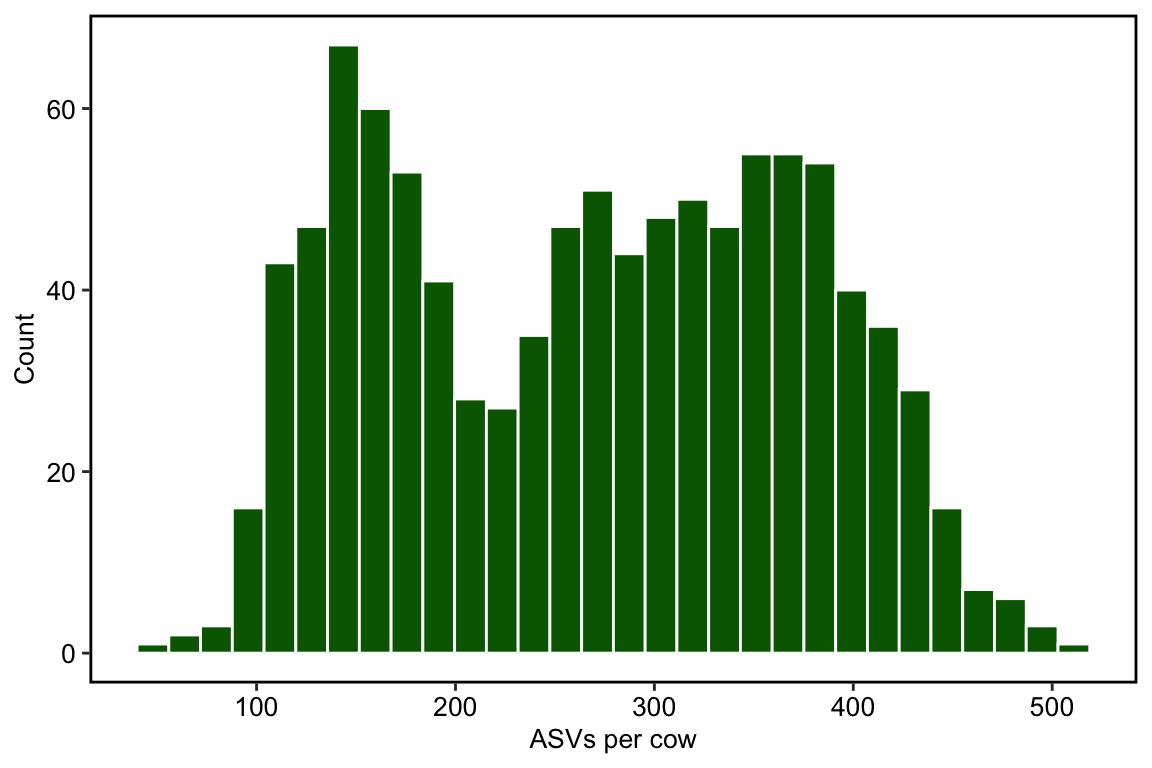
\includegraphics[width=1\linewidth,height=0.4\textheight]{exploratory_analysis_files/figure-latex/unnamed-chunk-3-1}

\hypertarget{richness-per-farm}{%
\subsection{Richness per farm}\label{richness-per-farm}}

\begin{Shaded}
\begin{Highlighting}[]
\NormalTok{plt\_richness\_per\_farm}
\end{Highlighting}
\end{Shaded}

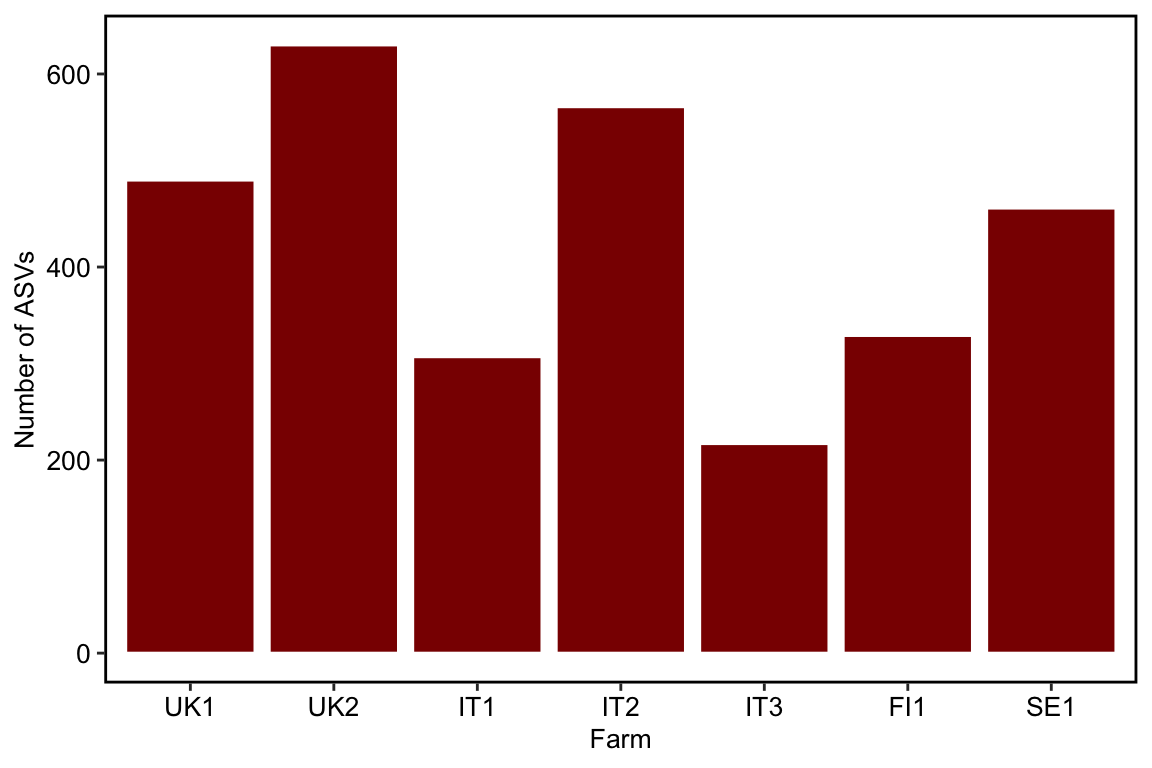
\includegraphics[width=1\linewidth,height=0.4\textheight]{exploratory_analysis_files/figure-latex/unnamed-chunk-4-1}

\hypertarget{richness-per-cow-within-farms}{%
\subsection{Richness per cow within
farms}\label{richness-per-cow-within-farms}}

\begin{Shaded}
\begin{Highlighting}[]
\NormalTok{plt\_richness\_per\_cow\_farm}
\end{Highlighting}
\end{Shaded}

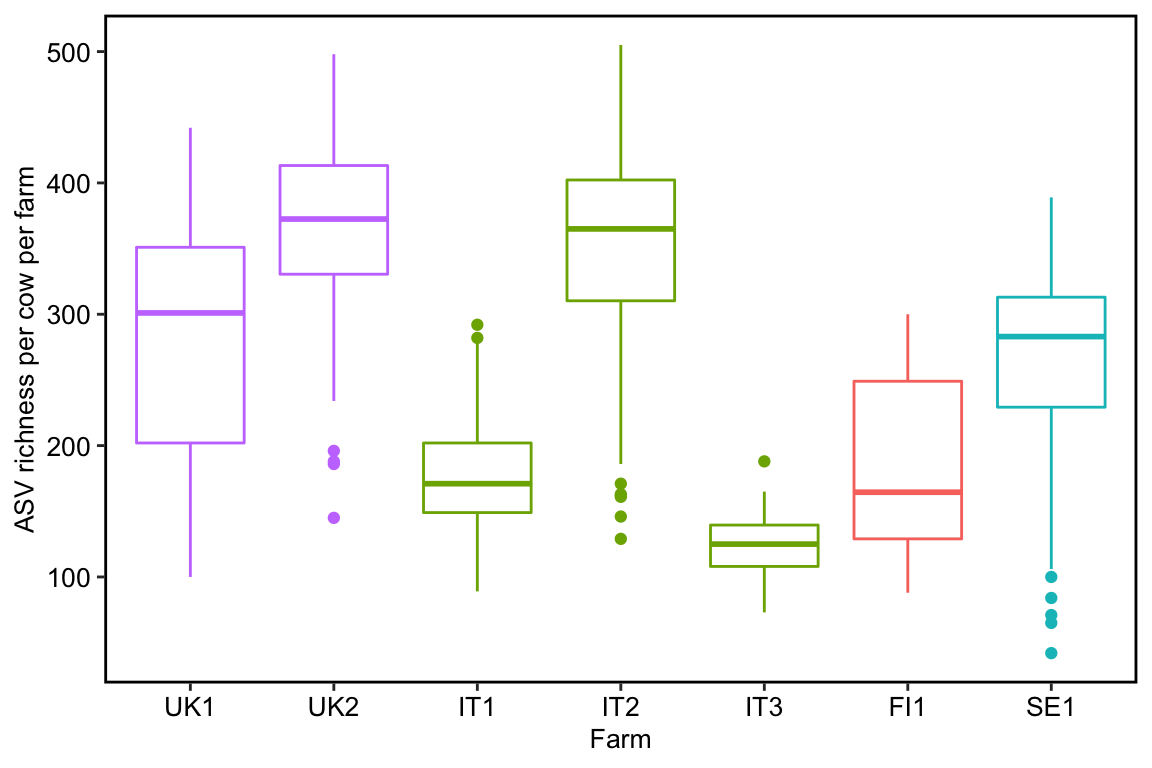
\includegraphics[width=1\linewidth,height=0.4\textheight]{exploratory_analysis_files/figure-latex/unnamed-chunk-5-1}

\hypertarget{asv-beta-diversity-between-farms}{%
\section{ASV Beta diversity between
farms}\label{asv-beta-diversity-between-farms}}

\begin{Shaded}
\begin{Highlighting}[]
\CommentTok{\# ASV Beta diversity between farms {-}{-}{-}{-}{-}{-}{-}{-}{-}{-}{-}{-}{-}{-}{-}{-}}
\NormalTok{ASV\_occurrence\_farm }\OtherTok{\textless{}{-}} 
\NormalTok{  ASV\_Core\_30 }\SpecialCharTok{\%\textgreater{}\%}
  \FunctionTok{select}\NormalTok{(}\SpecialCharTok{{-}}\FunctionTok{c}\NormalTok{(Cow\_Code)) }\SpecialCharTok{\%\textgreater{}\%}
  \FunctionTok{distinct}\NormalTok{(Farm, ASV\_ID) }\SpecialCharTok{\%\textgreater{}\%}
  \FunctionTok{mutate}\NormalTok{(}\AttributeTok{present=}\DecValTok{1}\NormalTok{) }\SpecialCharTok{\%\textgreater{}\%} 
  \FunctionTok{spread}\NormalTok{(ASV\_ID, present, }\AttributeTok{fill =} \DecValTok{0}\NormalTok{) }\SpecialCharTok{\%\textgreater{}\%}
  \FunctionTok{column\_to\_rownames}\NormalTok{(}\StringTok{"Farm"}\NormalTok{)}

\DocumentationTok{\#\# Using Jaccard {-}{-}{-}{-}}
\NormalTok{beta\_diver\_farms }\OtherTok{\textless{}{-}} \FunctionTok{as.matrix}\NormalTok{(}\DecValTok{1}\SpecialCharTok{{-}}\FunctionTok{vegdist}\NormalTok{(ASV\_occurrence\_farm, }\StringTok{"jaccard"}\NormalTok{))}
\FunctionTok{diag}\NormalTok{(beta\_diver\_farms) }\OtherTok{\textless{}{-}} \DecValTok{1}
\CommentTok{\# Heatmap}
\NormalTok{beta\_diver\_farms[}\FunctionTok{lower.tri}\NormalTok{(beta\_diver\_farms, }\AttributeTok{diag =}\NormalTok{ F)] }\OtherTok{\textless{}{-}} \ConstantTok{NA}
\NormalTok{beta\_diver\_farms\_m }\OtherTok{\textless{}{-}}\NormalTok{ reshape2}\SpecialCharTok{::}\FunctionTok{melt}\NormalTok{(beta\_diver\_farms) }

\NormalTok{plt\_J }\OtherTok{\textless{}{-}} \FunctionTok{ggplot}\NormalTok{(beta\_diver\_farms\_m, }\FunctionTok{aes}\NormalTok{(}\AttributeTok{x =}\NormalTok{ Var1, }\AttributeTok{y =}\NormalTok{ Var2, }\AttributeTok{fill =}\NormalTok{ value, }\AttributeTok{label=}\FunctionTok{round}\NormalTok{(value,}\DecValTok{2}\NormalTok{))) }\SpecialCharTok{+}
  \FunctionTok{geom\_tile}\NormalTok{() }\SpecialCharTok{+} 
  \FunctionTok{geom\_text}\NormalTok{(}\AttributeTok{color =} \StringTok{"black"}\NormalTok{, }\AttributeTok{size =} \DecValTok{4}\NormalTok{)}\SpecialCharTok{+}
  \FunctionTok{scale\_y\_discrete}\NormalTok{(}\AttributeTok{limits=}\NormalTok{rev)}\SpecialCharTok{+}
  \FunctionTok{scale\_fill\_gradient}\NormalTok{(}\AttributeTok{high =} \StringTok{"blue"}\NormalTok{, }\AttributeTok{low =} \StringTok{"light blue"}\NormalTok{, }\AttributeTok{na.value =} \StringTok{\textquotesingle{}white\textquotesingle{}}\NormalTok{) }\SpecialCharTok{+}
\NormalTok{  html\_figs\_theme\_no\_legend}\SpecialCharTok{+}\FunctionTok{theme}\NormalTok{(}\AttributeTok{axis.title =} \FunctionTok{element\_blank}\NormalTok{())}

\DocumentationTok{\#\# Using UniFrac {-}{-}{-}{-}}
\NormalTok{phylo\_tree }\OtherTok{\textless{}{-}} \FunctionTok{readRDS}\NormalTok{(}\StringTok{"local\_output/fitted\_asvs\_phylo\_tree.rds"}\NormalTok{)}
\NormalTok{tree }\OtherTok{\textless{}{-}}\NormalTok{ phylo\_tree}\SpecialCharTok{$}\NormalTok{tree}
\CommentTok{\# prune the tree}
\NormalTok{included\_asvs }\OtherTok{\textless{}{-}} \FunctionTok{unique}\NormalTok{(ASV\_Core\_30}\SpecialCharTok{$}\NormalTok{ASV\_ID)}
\NormalTok{unincluded }\OtherTok{\textless{}{-}}\NormalTok{ tree}\SpecialCharTok{$}\NormalTok{tip.label[}\SpecialCharTok{!}\NormalTok{tree}\SpecialCharTok{$}\NormalTok{tip.label }\SpecialCharTok{\%in\%}\NormalTok{ included\_asvs]}
\NormalTok{pruned }\OtherTok{\textless{}{-}}\NormalTok{ dendextend}\SpecialCharTok{::}\FunctionTok{prune}\NormalTok{(tree, unincluded)}
\NormalTok{unifracs }\OtherTok{\textless{}{-}} \FunctionTok{GUniFrac}\NormalTok{(ASV\_occurrence\_farm, pruned, }\AttributeTok{alpha=}\FunctionTok{c}\NormalTok{(}\DecValTok{0}\NormalTok{, }\FloatTok{0.5}\NormalTok{, }\DecValTok{1}\NormalTok{))}\SpecialCharTok{$}\NormalTok{unifracs}
\NormalTok{d\_UW }\OtherTok{\textless{}{-}} \DecValTok{1}\SpecialCharTok{{-}}\NormalTok{(unifracs[, , }\StringTok{"d\_UW"}\NormalTok{])}
\CommentTok{\# Heatmap }
\NormalTok{d\_UW[}\FunctionTok{lower.tri}\NormalTok{(d\_UW)] }\OtherTok{\textless{}{-}} \ConstantTok{NA}
\NormalTok{beta\_diver\_farms\_UF }\OtherTok{\textless{}{-}}\NormalTok{ reshape2}\SpecialCharTok{::}\FunctionTok{melt}\NormalTok{(d\_UW)}
\NormalTok{plt\_U }\OtherTok{\textless{}{-}} 
\FunctionTok{ggplot}\NormalTok{(beta\_diver\_farms\_UF, }\FunctionTok{aes}\NormalTok{(}\AttributeTok{x =}\NormalTok{ Var1, }\AttributeTok{y =}\NormalTok{ Var2, }\AttributeTok{fill =}\NormalTok{ value, }\AttributeTok{label=}\FunctionTok{round}\NormalTok{(value,}\DecValTok{2}\NormalTok{))) }\SpecialCharTok{+}
  \FunctionTok{geom\_tile}\NormalTok{() }\SpecialCharTok{+} 
  \FunctionTok{geom\_text}\NormalTok{(}\AttributeTok{color =} \StringTok{"black"}\NormalTok{, }\AttributeTok{size =} \DecValTok{4}\NormalTok{)}\SpecialCharTok{+}
  \FunctionTok{scale\_y\_discrete}\NormalTok{(}\AttributeTok{limits=}\NormalTok{rev)}\SpecialCharTok{+}
  \FunctionTok{scale\_fill\_gradient}\NormalTok{(}\AttributeTok{high =} \StringTok{"\#ff8c00"}\NormalTok{, }\AttributeTok{low =} \StringTok{"\#fff494"}\NormalTok{, }\AttributeTok{na.value =} \StringTok{\textquotesingle{}white\textquotesingle{}}\NormalTok{) }\SpecialCharTok{+}
\NormalTok{  html\_figs\_theme\_no\_legend}\SpecialCharTok{+}\FunctionTok{theme}\NormalTok{(}\AttributeTok{axis.title =} \FunctionTok{element\_blank}\NormalTok{())}

\CommentTok{\# \# Network representation}
\CommentTok{\# beta\_div\_net \textless{}{-} igraph::graph.adjacency(beta\_diver\_farms, mode = \textquotesingle{}undirected\textquotesingle{}, diag = F, weighted = T)}
\CommentTok{\# E(beta\_div\_net)$weight}
\CommentTok{\# V(beta\_div\_net)$color \textless{}{-} c(\textquotesingle{}blue\textquotesingle{}, \textquotesingle{}red\textquotesingle{}, \textquotesingle{}red\textquotesingle{}, \textquotesingle{}red\textquotesingle{}, \textquotesingle{}yellow\textquotesingle{}, \textquotesingle{}gray\textquotesingle{},\textquotesingle{}gray\textquotesingle{})}
\CommentTok{\# num\_ASV \textless{}{-} ASV\_data \%\textgreater{}\%}
\CommentTok{\#   group\_by(Farm) \%\textgreater{}\%}
\CommentTok{\#   summarise(ASV\_num=n\_distinct(ASV\_ID))}
\CommentTok{\# V(beta\_div\_net)$num\_ASV \textless{}{-} num\_ASV$ASV\_num }
\CommentTok{\# }
\CommentTok{\# \# pdf(\textquotesingle{}output/figures/beta\_div\_network.pdf\textquotesingle{},6,6)}
\CommentTok{\# pdf(\textquotesingle{}\textasciitilde{}/Dropbox (BGU)/Apps/Overleaf/Rumen microbiome coocurrence/beta\_div\_network.pdf\textquotesingle{}, 6, 6)}
\CommentTok{\# plot(beta\_div\_net, edge.width=E(beta\_div\_net)$weight*10, edge.color=\textquotesingle{}black\textquotesingle{}, layout=layout.circle, }
\CommentTok{\#      vertex.size=V(beta\_div\_net)$num\_ASV/40+20)}
\CommentTok{\# dev.off()}

\CommentTok{\# combine the two plots of beta diversity}
\CommentTok{\# png(filename = \textquotesingle{}local\_output/figures/beta\_diversity\_unif\_jacc.png\textquotesingle{}, width = 2000, height = 900, res = 300)}
\NormalTok{plt\_beta\_div }\OtherTok{\textless{}{-}} \FunctionTok{plot\_grid}\NormalTok{(plt\_J,plt\_U, }\AttributeTok{labels =} \FunctionTok{c}\NormalTok{(}\StringTok{\textquotesingle{}(A)\textquotesingle{}}\NormalTok{,}\StringTok{\textquotesingle{}(B)\textquotesingle{}}\NormalTok{))}
\CommentTok{\# dev.off()}
\end{Highlighting}
\end{Shaded}

Using Jaccard (A) and UniFrac (B)

\begin{Shaded}
\begin{Highlighting}[]
\NormalTok{plt\_beta\_div}
\end{Highlighting}
\end{Shaded}

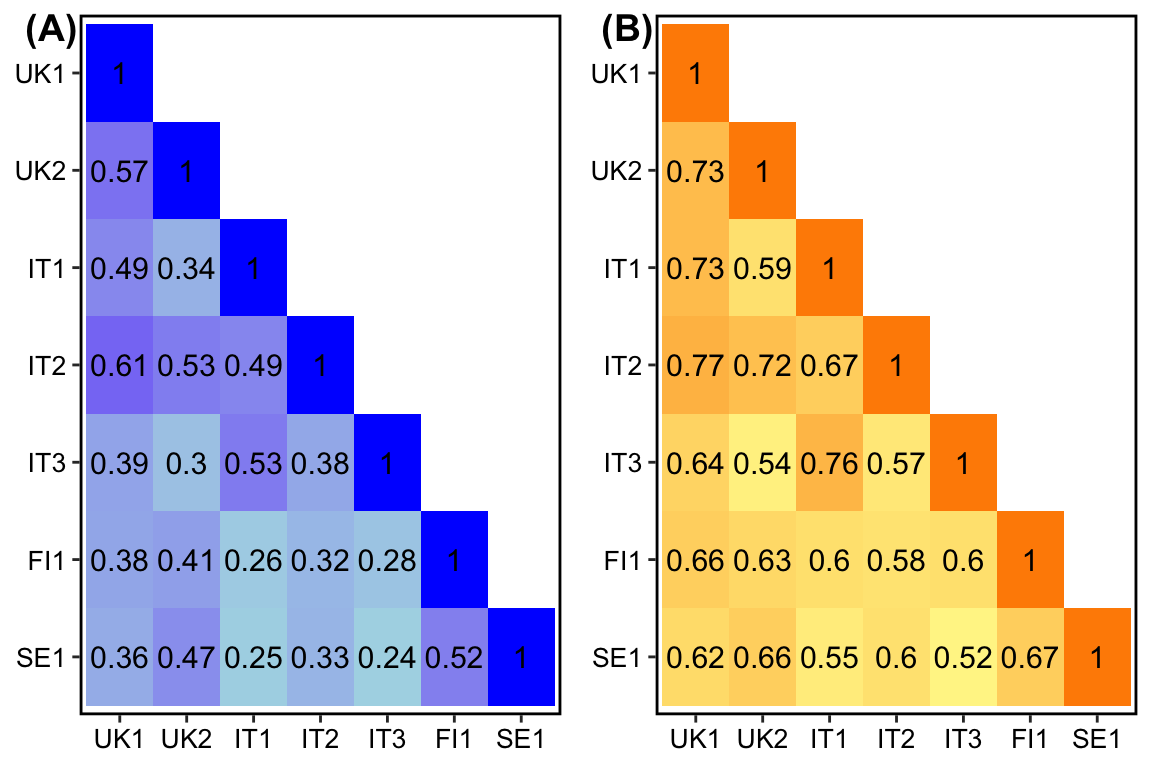
\includegraphics[width=1\linewidth,height=0.4\textheight]{exploratory_analysis_files/figure-latex/unnamed-chunk-7-1}

\hypertarget{multilayer-network}{%
\section{Multilayer network}\label{multilayer-network}}

\hypertarget{distribution-of-link-weights}{%
\subsection{Distribution of link
weights}\label{distribution-of-link-weights}}

\begin{Shaded}
\begin{Highlighting}[]
\NormalTok{multilayer\_unif }\OtherTok{\textless{}{-}} \FunctionTok{read\_csv}\NormalTok{(}\StringTok{\textquotesingle{}local\_output/multilayer\_unif.csv\textquotesingle{}}\NormalTok{)}
 \FunctionTok{ggplot}\NormalTok{(multilayer\_unif, }\FunctionTok{aes}\NormalTok{(weight, }\AttributeTok{fill=}\NormalTok{type))}\SpecialCharTok{+}
  \FunctionTok{geom\_density}\NormalTok{(}\AttributeTok{alpha=}\FloatTok{0.5}\NormalTok{)}\SpecialCharTok{+}
  \FunctionTok{labs}\NormalTok{(}\AttributeTok{x=}\StringTok{\textquotesingle{}Edge weight\textquotesingle{}}\NormalTok{, }\AttributeTok{y=}\StringTok{\textquotesingle{}Density\textquotesingle{}}\NormalTok{)}\SpecialCharTok{+}
  \FunctionTok{scale\_fill\_manual}\NormalTok{(}\AttributeTok{values =} \FunctionTok{c}\NormalTok{(}\StringTok{\textquotesingle{}blue\textquotesingle{}}\NormalTok{,}\StringTok{\textquotesingle{}orange\textquotesingle{}}\NormalTok{))}\SpecialCharTok{+}
\NormalTok{ html\_figs\_theme}
\end{Highlighting}
\end{Shaded}

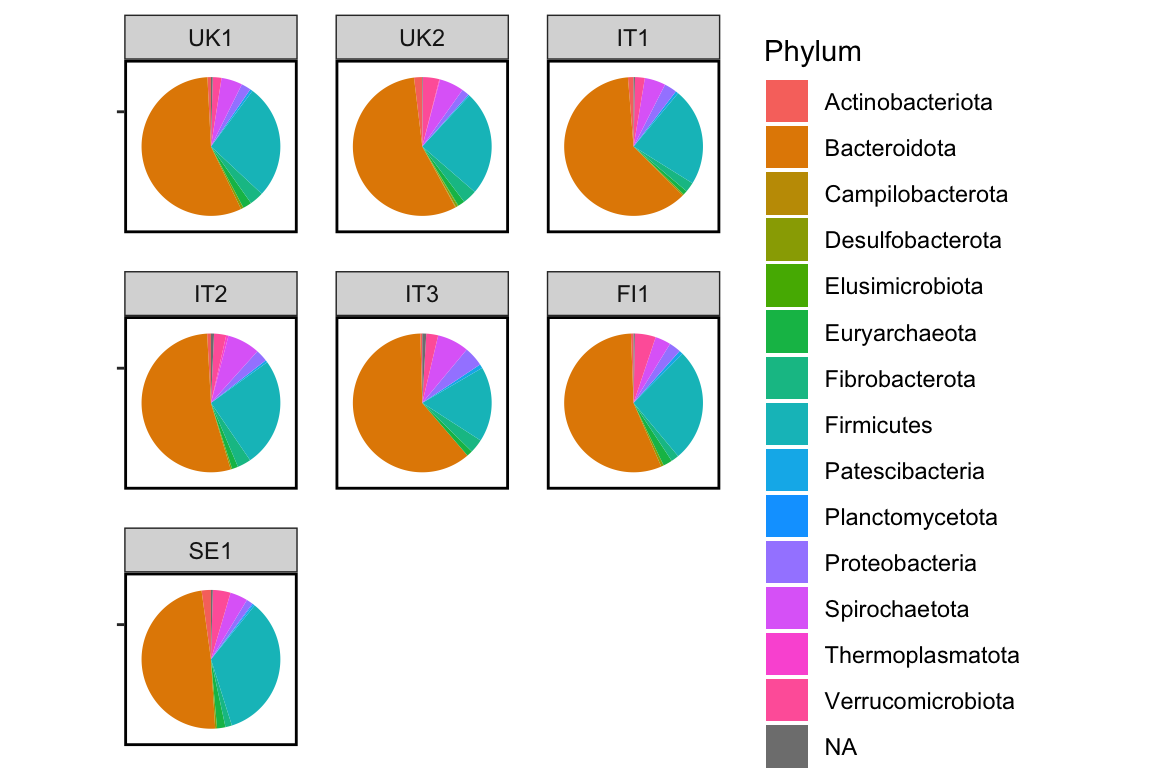
\includegraphics[width=1\linewidth,height=0.4\textheight]{exploratory_analysis_files/figure-latex/unnamed-chunk-8-1}

\end{document}
